%% bare_conf.tex
%% V1.4b
%% 2015/08/26
%% by Michael Shell
%% See:
%% http://www.michaelshell.org/
%% for current contact information.
%%
%% This is a skeleton file demonstrating the use of IEEEtran.cls
%% (requires IEEEtran.cls version 1.8b or later) with an IEEE
%% conference paper.
%%
%% Support sites:
%% http://www.michaelshell.org/tex/ieeetran/
%% http://www.ctan.org/pkg/ieeetran
%% and
%% http://www.ieee.org/

%%*************************************************************************
%% Legal Notice:
%% This code is offered as-is without any warranty either expressed or
%% implied; without even the implied warranty of MERCHANTABILITY or
%% FITNESS FOR A PARTICULAR PURPOSE! 
%% User assumes all risk.
%% In no event shall the IEEE or any contributor to this code be liable for
%% any damages or losses, including, but not limited to, incidental,
%% consequential, or any other damages, resulting from the use or misuse
%% of any information contained here.
%%
%% All comments are the opinions of their respective authors and are not
%% necessarily endorsed by the IEEE.
%%
%% This work is distributed under the LaTeX Project Public License (LPPL)
%% ( http://www.latex-project.org/ ) version 1.3, and may be freely used,
%% distributed and modified. A copy of the LPPL, version 1.3, is included
%% in the base LaTeX documentation of all distributions of LaTeX released
%% 2003/12/01 or later.
%% Retain all contribution notices and credits.
%% ** Modified files should be clearly indicated as such, including  **
%% ** renaming them and changing author support contact information. **
%%*************************************************************************


% *** Authors should verify (and, if needed, correct) their LaTeX system  ***
% *** with the testflow diagnostic prior to trusting their LaTeX platform ***
% *** with production work. The IEEE's font choices and paper sizes can   ***
% *** trigger bugs that do not appear when using other class files.       ***                          ***
% The testflow support page is at:
% http://www.michaelshell.org/tex/testflow/



\documentclass[conference]{IEEEtran}

\usepackage{listings}	
\usepackage{color}
\usepackage{graphicx}

\lstset{ %
language=C++,                % choose the language of the code
basicstyle=\footnotesize,       % the size of the fonts that are used for the code
xleftmargin=.2in,
numbers=left,                   % where to put the line-numbers
numberstyle=\footnotesize,      % the size of the fonts that are used for the line-numbers
stepnumber=1,                   % the step between two line-numbers. If it is 1 each line will be numbered
numbersep=5pt,                  % how far the line-numbers are from the code
backgroundcolor=\color{white},  % choose the background color. You must add \usepackage{color}
showspaces=false,               % show spaces adding particular underscores
showstringspaces=false,         % underline spaces within strings
showtabs=false,                 % show tabs within strings adding particular underscores
frame=single,           % adds a frame around the code
tabsize=2,          % sets default tabsize to 2 spaces
captionpos=b,           % sets the caption-position to bottom
breaklines=true,        % sets automatic line breaking
breakatwhitespace=false,    % sets if automatic breaks should only happen at whitespace
escapeinside={\%*}{*)}          % if you want to add a comment within your code
}

% *** GRAPHICS RELATED PACKAGES ***
%
\ifCLASSINFOpdf
  % \usepackage[pdftex]{graphicx}
  % declare the path(s) where your graphic files are
  % \graphicspath{{../pdf/}{../jpeg/}}
  % and their extensions so you won't have to specify these with
  % every instance of \includegraphics
  % \DeclareGraphicsExtensions{.pdf,.jpeg,.png}
\else
  % or other class option (dvipsone, dvipdf, if not using dvips). graphicx
  % will default to the driver specified in the system graphics.cfg if no
  % driver is specified.
  % \usepackage[dvips]{graphicx}
  % declare the path(s) where your graphic files are
  % \graphicspath{{../eps/}}
  % and their extensions so you won't have to specify these with
  % every instance of \includegraphics
  % \DeclareGraphicsExtensions{.eps}
\fi
% graphicx was written by David Carlisle and Sebastian Rahtz. It is
% required if you want graphics, photos, etc. graphicx.sty is already
% installed on most LaTeX systems. The latest version and documentation
% can be obtained at: 
% http://www.ctan.org/pkg/graphicx
% Another good source of documentation is "Using Imported Graphics in
% LaTeX2e" by Keith Reckdahl which can be found at:
% http://www.ctan.org/pkg/epslatex
%
% latex, and pdflatex in dvi mode, support graphics in encapsulated
% postscript (.eps) format. pdflatex in pdf mode supports graphics
% in .pdf, .jpeg, .png and .mps (metapost) formats. Users should ensure
% that all non-photo figures use a vector format (.eps, .pdf, .mps) and
% not a bitmapped formats (.jpeg, .png). The IEEE frowns on bitmapped formats
% which can result in "jaggedy"/blurry rendering of lines and letters as
% well as large increases in file sizes.
%
% You can find documentation about the pdfTeX application at:
% http://www.tug.org/applications/pdftex




% correct bad hyphenation here


\begin{document}
\title{Selective Vulnerability Analysis with\\
Binary Function Fuzzing (BFF)\\}

\author{\IEEEauthorblockN{Jeremy Solmonson}
\IEEEauthorblockA{School of Security Engineering\\
University of Colorado at Colorado Springs\\
Colorado Springs, CO 80922\\
Email: jsolmons@uccs.edu}}

\maketitle

\begin{abstract}
Vulnerability mitigation is essential for application development. Without the ability to timely find and mitigate software vulnerabilities, computer attacks will use the underlying weakness to take advantage of a computer system. Finding vulnerabilities as early as possible within the Software Development Life Cycle (SDLC), is the most cost efficient approach for application security. Unfortunately, most vulnerability analysis tools assess the software against the whole system, not individual parts of the program. As a result, the entire program must be completely written before the first vulnerability assessment is conducted. To integrate vulnerability identification earlier within the SDLC, a new tool named Binary Function Fuzzer (BFF) was developed. Integrating concepts from the Angr \cite{shoshitaishvili_sok:_2016} framework, the BFF tool allows software developers to integrate vulnerability identification within their unit tests and subsequently fixing the underlying issue. Additionally, bringing vulnerability identification to the individual developer enables faster mitigation strategies and stronger code ownership. 
\end{abstract}

\IEEEpeerreviewmaketitle

\section{Introduction}
The process of reducing the vulnerabilities within software is extremely time intensive because programs are becoming larger and more complex. These complex program require extra scrutiny as the underlying logic may not be well known or well tested. Without through testing, vulnerabilities may be overlooked and released into the final program. Additionally, commercial software developers are incentivized for releasing their products as quickly as possible, which can limit the rigorous testing needed to reach hard-to-find vulnerabilities. 

Exploitable vulnerabilities are extremely concerning for software development organizations. An exploitable vulnerability allows a computer attacker to use the underlying software in unintended methods. An attacker that can insert their own instructions as a substitute for the original programs to achieve Remote Code Execution (RCE). This can be considered the worst type of vulnerability as it allows the attack to execute their instructions up to the privileges of the application. For system services or processes that run with elevated permission, a RCE vulnerability allows the attacker complete control of the system. Testing for vulnerabilities on a continual basis reduces the potential for severely exploitable vulnerabilities.

To meet the organizational goals of balancing time with software quality, testing process is integrated into the earliest stages of software development known as unit tests. Unit tests allow the developer to ensure their features work as intended. However, unit tests do not usually include vulnerability testing. The problem with testing for vulnerabilities at the unit level is the time required to perform repetitive tests and observing unintended behavior. For large programs, execution from beginning to end can be severely time intensive. 

The problem becomes compounded after the software program is compiled and assembled into machine instructions. The ability to identify and execute the newly developed software feature becomes difficult due to the unique inputs required to execute the instructions. The majority of testing time isn't spent on testing the new feature, but instead traversing the branches within the program to execute the new feature. As a result unit tests become inefficient for vulnerability detection within binary analysis.

Despite the inefficiencies, developers usually write units tests to ensure the successful functionality of their code. Writing tests that intentionally perform failures is an after thought or non-existent practice. However, by writing tests that ensure a software fault results in graceful program termination should be an integral part of software development. Augmenting the testing procedures within a unit level fuzzer allows the developers to identify vulnerabilities in a timely manner. This paper will discuss a beta program called Binary Function Fuzzer (BFF), that can be used at the unit test level to search for vulnerabilities in individual units of code - see Figure 1. This allows security testing to be integrated at the lowest level of software development. By assisting software developers as they write the code, security vulnerabilities can be identified and fixed earlier within the SDLC. The final software product should have reduced the number of vulnerabilities.

\begin{figure}
  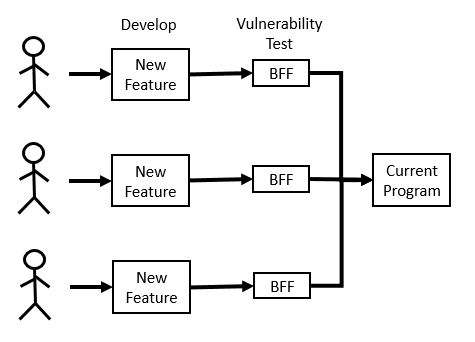
\includegraphics[width=\linewidth]{SDLC_BFF.JPG}
  \caption{Workflow with BFF}
  \label{fig:SLDC_BFF}
\end{figure}

The problem with fuzzing unit inputs is their unreliability due to manipulations by previous blocks of code. For instance, if a program first checks the user input for non-ascii characters and ensures the length is less than a maximum amount, then these characteristics are followed into the subsequent execution blocks. A unit level vulnerability fuzzer should observe these constraints and inject inputs that are consistent with the input the program would receive. Continually fuzzing inputs into individual functions poses environmental challenges. If the execution environment depends on specific variables, then the program needs to maintain the state of those variables in further testing. Take a file for instance, if the function enters with the current file pointer at a specific location within the file, the variable should returned to the same spot after the test completes. If the pointer is not returned, the future tests may be unreliable. This same logic is true for dynamically allocated memory, the current stack, and registers. Any block level test needs to be aware of saving the non-input variables and environment for further execution.

The BFF tool solves the above problems by providing a fuzzing capability that is integrated into unit level testing. This reduces the overall time required to test the system as the individual blocks of code are tested during development. Additionally, only the code up to the current function is analyzed. Alternative execution paths are not assessed. This allows the developer to better understand their integration into the current program. Further, by using a control flow graph with taint analysis, the BFF tool is able to identify the entry point into the function and symbolically execute with the desired parameters. 

This paper provides the following contributions:
\begin{itemize}
\item Demonstrates dynamic software vulnerability testing can be executed on selective function within a program
\item Introduces the BFF program for fuzzing individual functions within the resulting binary
\item Describes method that enables software developers to incorporate vulnerability identification within unit tests
\end{itemize}

\section{Background}
The main idea for this paper is to fuzz a select portion of a target program. By fuzzing a subset of the entire program, vulnerabilities can be identified in a deeper portion of the code. Usually, fuzzers that locate hard to find, or deep, bugs can only run a on select architectures due to their unique design. The scalability of these tools can be overcome by analyzing the resulting file. 

Implementing security testing with every phase of the SDLC creates resilient code. Unfortunately, the tools available to a development team to implement security coding practices are limited. This is especially true during the earlier phases of the SDLC. The ability to detect and fix a vulnerability is less expensive if the problem is found earlier with the SDLC \cite{tuteja_research_2012}. By implementing security testing tools earlier with the development process, the overall program will be more resistant to vulnerabilities. Figure 1 demonstrates the workflow of implementing security testing after a new feature is developed, but before it is implemented into the current program. The workflow pushes security testing to the lowest level possible - the individual developer. By having the developer responsible for their own security testing, better code is developed. Further, the results are reviewed by the individual developer for their own feature. This allows the to learn from their past mistakes and take corrective action to prevent future vulnerabilities. 

\begin{figure}
  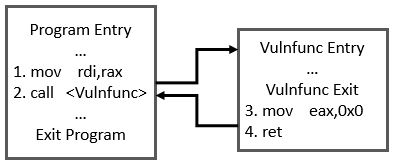
\includegraphics[width=\linewidth]{Program_flow.JPG}
  \caption{Execution of a function}
  \label{fig:Program_Flow}
\end{figure}

Functions are unique in the execution flow of a binary program due to the need to save the return address. When a function is called within a program, the program saves the current states of the execution for later use, sets arguments to the newly called function, and begins executing at the entry point of the function. Figure 2 visualizes the relationship between the original program and a function call. Item 1. in Figure 2 is the setting of arguments for prior to calling the vulnfunc function on the next line 2. After the function is executed, the original program continues execution at the next instruction. A function is easily identified in binary analysis with the "call" command. Once a function has completed its execution and is ready to exit, the reverse of the setup process is accomplished. The return value is saved into a register for the original execution to use - see line 3. Additionally, the return address is recalled to return execution prior to the function call and machine state is restored - see line 4. This allows for a function to be considered a stand-alone execution and only relies on the original program for function arguments. This stand-alone properties allows for functions to be imported into other programs, and is compatible as long as the same type of arguments are supplied to the function. A fuzzer can import the same function and generate fuzz to supply to the function arguments. Doing so allows for individual features of the program to be fuzzed without the need to execute the entire program. 

To abstract a portion of the program into a subset of the program requires Function Call Interception (FCI) [cite]. This allows a second program to use instrumentation by substituting, or modifying, the underlying main program. By modifying the main program, a developer can gain deep insight into a portion target program behavior. FCI allows the developer to substitute instructions or data variables to alter the main programs execution. In the BFF program, FCI is implemented through a third party program called Angr which in a binary analysis framework. Angr allows function to be executed as stand-alone applications though symbolic execution. While symbolic execution is not necessary for the BFF tool to operate, it does provide advantages for future tool expansion.  While FCI is used for mostly debugging purposes, it can be extended to fuzzing.

Fuzzing is injecting semi-valid inputs into a target program with the intent to find bugs. This technique has been an area of recent research [cite] to find unknown vulnerabilities. Fuzzing is known to find vulnerabilities by identifying a crash within the program. The crash occurs because the return address no longer executes at the proper location. Instead, a crash occurs that allowed the user to overwrite the return address location. If identified correctly, an attacker can set the return address to exploit the weakness and execute chosen instruction. One of the problems with fuzzing is executing deep into the program to find hard to reach bugs. This issue has been partly solved with symbolic execution and constraint solvers[cite]. However, the problem still remains due to resource exhaustion [cite]. As programs become larger and more complex, more resources are needed to fuzz deeper into the program. One method to overcome this challenge is to allow the developer to identify areas of interest to fuzz. By fuzzing a portion of the program, the time needed to test can be significantly reduced. Further, this technique can be integrated into the software development process. Fuzzing a software feature as it becomes available will lead to higher quality coding practices. 

To assist the developer further, taint analysis is able to identify user inputs and mark, or taint, them as untrusted. Following these variables within a program can identify execution paths that leads to user triggered bugs. The execution paths can be traced using static or dynamic analysis. Static analysis allows the tester to view the underlying program logic, commonly through a disassembler. The program logic can be further analyzed through a Control Flow Graph (CFG). The combination of static analysis and a CFG allows the user to view program execution through the basic blocks of code. As an analogy, the static analysis CFG view provide a road-map of the underlying program logic, while dynamic analysis drives down the individual roads. Dynamic analysis assesses a program during execution and provides relevant information back to the user. During dynamic analysis a program can be halted, modified by changing memory contents or registers, and then continue execution. This allows a user to assess different combinations to trigger function execution. By combining a control flow graph and tainting the input variables, a user is able to visually identify areas of potential concern within an application. Then using dynamic analysis, these input paths can be executed and observed in real time to provide further information. 

The one issue with dynamic analysis is finding the right combination of inputs to execute a specific path. To overcome this challenge, symbolic execution with constraint solvers is used to identify inputs for path execution. By using a constraint solver to find the conditions for branch execution, a single execution path can be identified. This enables a repeatable process to narrow down a source of program feature. One tool in recent research that performs this activity is Angr [cite]. Angr is a binary analysis framework that is integrates into the python programming interface. By using this existing framework, a program can be created to limit the scope of binary execution to a single path.

Combining the above techniques allows a software developer to fuzz their individual software feature. The function is first extracted through FCI by identifying the function entry point. Then function arguments are substituted with fuzz identified by the software developer. Next the program is dynamically executed with the fuzz and the return address is recorded. Optionally, taint analysis allows the inputs to be specially crafted according to the specifications of the program. Finally, symbolic execution can record the paths within the function execution to determine if a new path was taken or if a different return address was executed. 

\section{Related Work}
Fuzzing is an expansive topic that has received much attention over the past few years. [cite] While most research focuses on the performance of the fuzzer, that has been little research in new techniques that improve the fuzzing process. Angr was developed as a framework to stimulate new techniques in binary analysis. While Angr is a significant contributor to this paper, the research differs with a focus on fuzzing. Angr enables the function extraction through symbolic execution, while BFF focuses on fuzzing the results and reporting any vulnerabilities. Driller [cite] is a fuzzing tool that uses symbolic execution to identify hard to find vulnerabilities. It does this by symbolically executing the entire program. Ideally, BFF could be used as an add-on the the driller functionality. Concolic execution based on control-flow analysis [cite] has show significant progress in reducing the time to identify fuzzing inputs that leads to new execution paths. This feature is desirable when testing entire programs or individual functions. The inputs can be adjusted to the previous output and is considered the next phase into BFF development. Eliminating undesired inputs is essential in executing a fuzzer as efficiently as possible. TaintTrace flow tracing with dynamic binary rewrite [cite] has shown how tainting untrusted input can be used within binary analysis. While sanitizing untrusted input is a key defense within software applications, identifying the upper and lower bounds of the input provides great vale for fuzzing. By reducing the inputs to the minimal set of allowed values, allows the fuzzer to examine only valid inputs. A combination of static program analysis assisted with dynamic analysis will allow for further vulnerability discovery [cite]

\section{Experiment Design}

\begin{figure}
  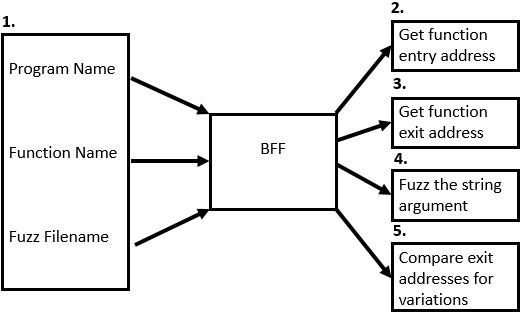
\includegraphics[width=\linewidth]{HowBFFWorks.JPG}
  \caption{BFF Concept}
  \label{fig:BFF_CONCEPT}
\end{figure}

%The experiment is designed to compare full program fuzzers against feature specific fuzzers such as BFF. The result is to capture accuracy and efficiency of the fuzzer technology in terms of vulnerability identification and time of detection. By comparing the state-of-the-art fuzzers on these two metrics, we can find the overall performance increase (or decrease) each fuzzer exhibits. As there are different categories of various fuzzers, the experiment will focus on vulnerabilities that result in remote code execution. The fuzzers were selected based on age (updated in last 2 years), open source, run on x86\_64 architecture, and able to execute Linux Executable and Linkable Format (ELF).

The experiment is designed to compare custom and existing function in a program that are extracted for fuzzing. GCC, an open source C compiler, provides common functions that accept parameters and produce an output. GCC if very common for software development and is the compiler chosen for this experiment. GCC provided functions that currently integrate within the BFF tool are printf, puts, atoi, atol, atof. These functions have the sole parameter as a string of characters and are the chosen functions for analysis. Also, a custom function was built, vulnfunc, that performs a known buffer overflow with strcpy. This custom function is ideal as it meets the BFF tool specifications and demonstrates applicability to fuzzing custom functions. The result of this experiment is to identify any limitations that fuzzing could have on Function Call Interception.  By identifying the success or failure of fuzzing within FCI, future experiments can be conducted to make the technique more effective and efficient. 

To identify a function with in a binary, static analysis plays a key roll by comparing the function name to the virtual address. To assist with this identification, a Control Flow Graph (CFG) is used with analysis of the execution path. The CFG created by Angr identifies the function name to function address translation within BFF. By extrapolating the memory address within the application, its possible to save the program state prior to execution of the function. The current state of the program can be modified based on the user input. Using this  feature in conjunction with Angr's function callable method, we are able to execute the function by providing function arguments. In essence, this has created a stand-alone program that only executes the function and records the results. As our  tools is only interested in remote code execution, the state of the return address is most important. The downside of Angr is the use of symbolic execution for program flow. Symbolic execution substitutes concrete variables with symbolic variables to execute both execution paths. While ideal for larger programs, this features is not needed for this tool. However, the symbolic return address on a "good" execution remains constant. As a result, we an substitute the symbolic return address as the real return address, which will not impact the results of the program. When the return address is overwritten, such as a buffer overflow, the program returns a different symbolic address. By comparing the "good" symbolic return address to the "bad" symbolic return address, we can conclude if a vulnerability exists.

BFF was designed to allow a developer to fuzz a specific function within a program - see figure 3. The developer would provide a file with function arguments to execute as the "fuzz" inputs (3.1). Based of a known good execution run, supplied by the developer, the BFF application would the get the function entry address (3.2) and function return address (3.3). The return address will be compared against all future runs. By repeatedly fuzzing various arguments within the function (3.4), the result my be different if the return address was incorrectly calculated. This would indicate an input was able to take control or modify the the return address. As a result, the return address is compared against the known good return value (3.5).  

While we can conclude if a vulnerability exists within an application, none of the fuzzing tools can conclude if a vulnerability doesn't exist. While fuzzing has it's limitation, we can assess the false positive rate against reliable code. By testing secure code, we can determine if the fuzzer is prone to revealing false positives. False positives can be a result of a combination of various circumstances. While fuzzers should report almost no false positive, the test is necessary to gauge the effectiveness of the fuzzer. To thwart against a fuzzer that reports every application is vulnerable, we tested against known good programs. This two part process was to minimize the possibility of a false negative. 

\begin{figure}
\begin{lstlisting}
// Vulnerable Test function
int vulnfunc(char * test){
	char vulnstr[16];
	strcpy(vulnstr, test); // Vulnerability is here
	return 0;
}

int main(int argc, char * argv[]) {
	// call vulnerable function and return result
	if(!vulnfunc(argv[1])) {
	    printf("success\n"); }
	return 0;
}
\end{lstlisting}
\caption{Vulnerable Code Example}
\end{figure}

\subsection{Test Case}
Figure 6 is a simple program that contains a buffer overflow. The design of the program is for the user to pass a string as a program parameter and the user supplied string is then copied to an in memory location. If the copy was successful, then a "success" message is printed to the screen. This simple program demonstrates taking control of return address by overwriting memory beyond the bounds of the allotted memory. Fuzzing this program with a traditional fuzzer would have the same effect as a function fuzzer such as BFF. The overhead to execute the function compared to the regular program is minimal. However, if we simulated additional code placed prior to lines lines 10 and lines 12, then fuzzing a function would be more advantageous.  

\section{Results}
The Binary Function Fuzzer was executed on select functions provided by the GCC library. The functions were selected based on their sole parameter as a string type. No noticeable timing differences were observed on the tested functions. In all cases, the BFF tool was able to identify the entry point to the function within the binary - see figure 5. By finding the function entry point, the arguments of he function can also be identified.  Using the entry point, BFF substituted the actual argument for the fuzzed input supplied by an input file. The input file used was a small list of strings that may trigger a vulnerability. Upon triggering a potential vulnerability, the BFF tool reported the input that triggered the issue and provided a notification through the console output. If no vulnerability was observed, then the tool reported no issues. In all cases, except for the test case, the tool did not report any vulnerabilities.

\begin{table}
 \begin{tabular}{|c|c|c|c|} 
 \hline
 & Entry Point Found & Function Fuzzed & Vuln Found  \\ 
 \hline
   vulnfunc & 
   Yes & 
   Yes & 
   Yes \\
\hline
   printf & 
   Yes & 
   Yes & 
   No \\
\hline
   puts & 
   Yes & 
   Yes & 
   No \\
\hline
   atoi & 
   Yes & 
   Yes & 
   No \\
\hline
   atol & 
   Yes & 
   Yes & 
   No \\
\hline
   atof & 
   Yes & 
   Yes & 
   No \\
\hline
\end{tabular}
\bigskip
\\
\caption{BFF Results}
\end{table}

The experiment showed custom functions and existing functions within and executed as stand alone programs. This observation allows the features to be executable as stand-alone programs and testing can be accomplished on the individual features. In this example the feature was fuzzed for potential vulnerabilities by observing changing behaviors in the return address. The only program that observed a vulnerability was the custom vulnfunc function that was known to have a buffer overflow. The tested functions that are included in the gcc library did not demonstrate any vulnerabilities. This is expected behavior as our fuzzing file had limited input strings - see Table 1. While the BFF did not observe any vulnerabilities in the gcc tested functions, this does not eliminate the possibility that a vulnerability exists. Nevertheless, both custom functions and pre-existing functions were able to be fuzzed as stand-alone features. The observation that all of the functions were successfully fuzzed demonstrates that selective execution can be used as a fuzzing technique. 

While not included as part of the experiment, it was observed that functions do not need to be executed concretely for the function fuzzing technique to be successful. The symbolic variables, including the return address, can behave similarly as if the program was executed concretely. The benefit of symbolic execution provides an abstraction to substitute input variables. This allows a program to select branch execution and execute other paths of interest. Further, the symbolic execution property could lead to further automation by expanding into sub-functions. 

\begin{figure}
\begin{lstlisting}
call   710 <puts@plt>
call   730 <strlen@plt>
call   750 <printf@plt>
call   780 <atoi@plt>
call   720 <atof@plt>
call   770 <atol@plt>
\end{lstlisting}
\caption{Select output from objdump}
\end{figure}

The result of the above analysis introduces a new framework that can be used to identify vulnerabilities within the Software Development Life Cycle. Instead of performing holistic vulnerability tests on the entire completed program, vulnerability tests can be conducted on the individual features of a given program. Source code can be downloaded from the github repository located at https://github.com/jsolmons/BFF The following are recommendations as improvements to the secure coding process.

\subsection{Features should be written as stand-alone functions}
Stand-alone functions provides the ability to insert functionality into multiple pieces of code while only writing the function once. This characteristic allows software developers to not only reuse code, but also upgrade the function without impacting the usability of the rest of the program. If one function of code contains a vulnerability, that function can be upgraded, rewritten, or removed to ensure the security of the remainder of the program. As a counter example, if the feature was not written within a specific function, but instead across multiple functions, the ability to upgrade and meet security requirements could be significant hindered. As a result, features should be implemented as stand alone functions and called for execution as needed. 

\subsection{Fuzzing should be conducted on individual functions}
Prior to introducing a new feature into the overall program, the new feature should be tested for vulnerabilities. By security testing each feature before integration, the security of the larger program is preserved. Fuzzing is a proven method to find exploitable vulnerabilities within programs [CITE]. While most fuzzers rely on executing the entire program, fuzzers can provide the capability to fuzz individual features of a program. The BFF tool provides a capability, albeit limited capability, to fuzz a feature after the it is fully developed. The ability to perform feature fuzzing resides on the stand-alone property of the individual feature. Extracting the individual feature and fuzzing that section of code without executing the entire program. This provides a more efficient and effective fuzzing technique. 

\subsection{Fuzzing should be conducted while the code is developed}
While the final feature should be fuzzed before being integrated into the larger program, the feature should also be fuzzed as its being developed. By performing these tests during development, the software developer can alter their underlying logic before completing their feature. As long as the feature under development is able to accept a parameter, it can be fuzzed during development. BFF has shown this is possible, even with limited use. By performing vulnerability testing early and fixing problematic code as soon as possible, eliminates issues in future code that relies on previous code. This allows for a secure rapid development process without excessively impacting the individual developer. 
 

\section{Threats to Validity}
The BFF tool uses symbolic execution with a symbolic return address to determine if the function returned from a normal execution path. It's possible the symbolic execution engine decided to allocate an alternative memory location for execution. As a result, this would have a significant impact on the results. Fortunately, we did not see this within our tests, but this could happen on an alternative symbolic engine. 

While similar tools were selected for comparable testing, some tools are designed to execute faster in different environments. The tools we selected against may not have been ideal for our chosen environment. If the tests were to run on a different architecture, compilers, or operating system, then the results may have significant variation. 

\section{Future Work}
The BFF tool only examined functions within a binary application. While directly applicable to customized sections within a software application, this has a broader impact including exported functions and shared libraries. Other applications may use similar features that can take advantage of fuzzing individual sections of code, such as start and stop ranges. By providing a start and stop range, the fuzzer is no longer limited to functions, instead it can fuzz anywhere within the target program. This provides more execution paths and unique scenarios to enhance security practices. 

The BFF tool only provides basic types for argument inputs (i.e. strings). The advanced types such as structures, pointers, and unions would be advantages as programmers become more abstracted. Providing this capability would require an enhancement to the fuzzing input file to supply the correct types to the function arguments. If a function argument is also the expected return result, then a memory range needs to be assigned to the program and stored after the function completes. The ability to process different types of data and functions can make fuzzing tools more universal. 

To gain a higher fidelity of test results, modifying the fuzzing tool to catch other types of vulnerabilities is desirable. The BFF tool only looks for a specific type of vulnerability, remote code execution. Other vulnerabilities such as memory leaks and format string errors could be identified by examining the functions output. This can be tested against a broader category of NIST Juliet test suite to examine other vulnerable applications. 

The BFF tool is a single threaded application and our goal was to test similar tools. Most fuzzers that perform dynamic analysis have the option of utilizing additional cores of processing. The BFF tool can be upgraded to accept multiple instances of dynamic fuzzing. 

\section{Conclusion}
The results from our test case proved the ability to fuzz individual components within a larger program. Breaking down a larger program into subcomponents provides scalability and ownership over the features within a given program. This advancement will allow developers to perform security tests as they develop code for their target program. The BFF tool provides a mechanism to fuzz individual functions which comprise of a much larger program. The speed at which the fuzzer increases performance is directly related to the execution time of the target program. By examining only areas of interest within the target program, we are able to utilize execution of specific targeted function. By introducing the BFF program we hope to inspire future fuzzing techniques that will assist with vulnerability prevention. Providing security tools to developers as they write their code will reduce the amount of vulnerabilities and improve secure coding practices. 

% references section
\nocite{*}
\bibliographystyle{IEEEtran}
\bibliography{Final}

\end{document}


